\documentclass[preprint,12pt]{elsarticle}
\usepackage{amsmath,amssymb,amsthm,amsfonts}
\usepackage{stix}
\usepackage{booktabs,graphicx,xcolor,float,array}
\usepackage[colorlinks=true,linkcolor=blue,citecolor=blue,urlcolor=blue]{hyperref}
\newtheorem{theorem}{Theorem}
\newtheorem{result}{Result}
\theoremstyle{remark}
\newtheorem{remark}{Remark}
\newfloat{algorithm}{tbp}{loa}
\floatname{algorithm}{Algorithm}
\newcommand{\todo}[1]{\textcolor{red}{\textbf{[TODO: #1]}}}

\newcommand{\step}[1]{\par\noindent\hangindent=1.5em\hangafter=1\textbf{Step #1.}\ }
\setlength{\emergencystretch}{2.5em}
\newcommand{\repo}{\url{https://github.com/mossaiby/iHaar}}
\newcommand{\archive}{\url{https://github.com/mossaiby/iHaar/releases/tag/v1.2}}
\journal{Engineering Analysis with Boundary Elements}

\begin{document}
\begin{frontmatter}
\title{Fast solvers on arbitrary grids for Haar wavelet collocation:
sharp-interface phase-field computations and adaptive elastostatics}

\author[inst1]{Farshid Mossaiby\corref{cor1}}
\ead{mossaiby@eng.ui.ac.ir}
\cortext[cor1]{Corresponding author}
\affiliation[inst1]{organization={Department of Civil Engineering, University of Isfahan},
            city={Isfahan}, postcode={81744-73441}, country={Iran}}

\begin{abstract}
The Haar wavelet collocation method (HWCM) is popular in engineering because it is easy to derive and
to program. In two and three dimensions, however, it is usually solved through large dense matrices, and
it is limited to second-order accuracy. We show that these limitations disappear when the method is
written in terms of nodal values, where it becomes midpoint quadratic-spline collocation. An exact
three-term relation turns the dense HWCM matrices into tridiagonal ones, and we prove that the resulting
second-derivative operator has real, simple and nonpositive eigenvalues on every strictly increasing
grid. Fast diagonalization, which reduces problems on tensor grids to a few dense matrix products, is
therefore always well defined, including on adaptively refined grids. In floating-point arithmetic it
was backward stable on random and adversarial grids, and an inexpensive check guards against failure. On uniform grids, a correction that costs nothing extra
raises the accuracy to fourth order for zero-flux conditions. Building on this, we present Allen--Cahn
and Cahn--Hilliard solvers that conserve mass exactly, satisfy a modified-energy law, and resolve
interfaces with about four nodes across the transition layer. We also present a plane elastostatics
solver for compressible materials with prescribed displacements and tractions, whose automatic
refinement recovered the optimal convergence rate at the tested corner singularities. In a benchmark
against biquadratic finite elements on identical grids, the method needed about a quarter of the
unknowns. The code that reproduces every result is openly available.
\end{abstract}

\begin{keyword}
Haar wavelet collocation \sep spline collocation \sep fast diagonalization \sep graded grids \sep Cahn--Hilliard \sep
sharp interfaces \sep corner singularities \sep adaptive refinement
\end{keyword}
\end{frontmatter}

%==========================================================================
\section{Introduction}
%==========================================================================
The Haar wavelet collocation method (HWCM)~\cite{chen1997haar,lepik2005numerical,lepik2011solving,lepik2014book}
is widely used in applied mechanics for beams, plates, shells and functionally graded
structures~\cite{majak2015accuracy,majak2015convergence,majak2018higher}. The highest derivative of the
unknown is expanded in Haar functions, the lower derivatives follow by exact integration, and the
equation is enforced at cell midpoints. Higher-order variants~\cite{majak2018higher,ratas2021solving} and
graded grids based on non-uniform Haar functions~\cite{dubeau2004nonuniform,lepik2008nonuniform,oruc2019nonuniform}
are available. In two dimensions, however, all equations are usually assembled into one dense matrix of
size $N^2\times N^2$, which becomes impractical beyond about $64\times64$ cells. Graded grids must be
designed by hand, and for nonlinear time-dependent problems no stability results are available.

In terms of nodal values, HWCM is midpoint quadratic-spline collocation
(QSC)~\cite{houstis1988quadratic,christara1994quadratic,christara2006optimal}, and it uses the same
functions as quadratic isogeometric collocation~\cite{auricchio2010isogeometric,schillinger2013isogeometric}.
On tensor grids, separable problems can be solved by fast diagonalization~\cite{lynch1964direct}, which
reduces two- and three-dimensional problems to dense matrix products and fast transforms that run
efficiently on CPUs and GPUs. It requires each one-dimensional operator to be diagonalizable with real
eigenvalues. For
symmetric finite-element and isogeometric Galerkin operators this is automatic~\cite{sangalli2016isogeometric}.
Collocation operators are generally not symmetric, and for them the property has to be proved. For
Hermite-cubic orthogonal spline collocation it is known~\cite{dyksen1987tensor,sun1999spectral}, and it
underlies the matrix decomposition algorithms of Bialecki and Fairweather~\cite{bialecki1995matrix,bialecki2011matrix}.
For QSC, fast solvers exist on uniform grids~\cite{christara2002fast}. To our knowledge, the property has
not been established for midpoint QSC, equivalently nodal HWCM, on arbitrary graded grids. There, the
collocation operator is not symmetric and is not symmetrized by quadrature weights, so a different
argument is needed. Without a guarantee, fast diagonalization on adaptively refined grids could fail.

This paper closes that gap and builds on it. Our central result (Theorem~\ref{thm:spectrum}) is that, on
every grid, the HWCM second-derivative operator has real, distinct and nonpositive eigenvalues, so the
fast solver always applies. We check its numerical reliability (Section~\ref{sec:robust}) and use it in
three engineering settings: fast solution on arbitrary graded grids, Allen--Cahn and Cahn--Hilliard
computations with thin interfaces, which conserve mass exactly, and elastostatics of compressible
materials with traction boundaries and automatic, including local, refinement at corner singularities.
Table~\ref{tab:closest} compares the method with the closest existing approaches. The main text keeps
the mathematics to what is needed to use the method; derivations are in the appendices, and formal
statements and proofs in Part~A of the Supplementary Material. The code is available at \repo.

\begin{table}[t]\centering\footnotesize
\caption{Comparison with the closest spline-collocation approaches, to the best of our knowledge. ``Spectrum'' refers to the one-dimensional collocation operator used by fast diagonalization or matrix decomposition.}\label{tab:closest}
\begin{tabular}{>{\raggedright\arraybackslash}p{0.14\textwidth}>{\raggedright\arraybackslash}p{0.175\textwidth}>{\raggedright\arraybackslash}p{0.13\textwidth}>{\raggedright\arraybackslash}p{0.23\textwidth}>{\raggedright\arraybackslash}p{0.17\textwidth}}
\toprule
Method & Trial space and collocation points & Grids & Spectrum & Fast solver\\
\midrule
Classical HWCM~\cite{lepik2011solving,oruc2019nonuniform} & integrated Haar ($C^1$ quadratics); midpoints & uniform or a~priori graded & not analysed & none (dense $N^2\times N^2$ solve)\\\addlinespace
Hermite-cubic OSC~\cite{dyksen1987tensor,sun1999spectral,bialecki1995matrix} & $C^1$ cubics; two Gauss points per cell & partitions as in the cited works & real, distinct eigenvalues established & matrix decomposition (MDA), FFT on uniform grids\\\addlinespace
QSC~\cite{houstis1988quadratic,christara2002fast,christara2006optimal} & $C^1$ quadratics; midpoints (optimal variants perturbed) & uniform; non-uniform analysed for convergence & symmetric with trigonometric eigenvectors on uniform grids & FFT and MDA on uniform grids\\\addlinespace
Quadratic IGA collocation~\cite{auricchio2010isogeometric,schillinger2013isogeometric,delorenzis2015isogeometric} & B-splines; Greville or superconvergent points & arbitrary knots; local refinement & not established for collocation; Galerkin pencils symmetric~\cite{sangalli2016isogeometric} & direct or Krylov; FDM for the Galerkin counterpart\\\addlinespace
This work & $C^1$ quadratics; midpoints & arbitrary graded tensor grids & real, simple, nonpositive on every grid (Theorem~\ref{thm:spectrum}) & FDM on any tensor grid, with a safeguard; DCT/DST on uniform grids\\
\bottomrule
\end{tabular}
\end{table}

%==========================================================================
\section{The method}\label{sec:method}
%==========================================================================
\subsection{From Haar wavelets to nodal values}
Let $a=t_0<t_1<\dots<t_N=b$ be the grid, with cells of width $h_k$ and midpoints $m_k$. HWCM expands
$u''$ in Haar functions and integrates twice. On a given grid, the Haar functions span exactly the
functions that are constant on each cell, so the Haar coefficients carry the same information as the
cell values $c_k$ of $u''$. Integrating twice gives piecewise quadratics with continuous slopes, that is,
quadratic splines. We use the values $U_k$ at the cell midpoints, which are the HWCM collocation values,
as unknowns.

The key observation is that the nodal values and the cell values of $u''$ are linked by an exact
three-term relation, derived in~\ref{app:identity}:
\begin{equation}\label{eq:identity}
\mathbf L\mathbf U+\mathbf b=\mathbf A\mathbf c,
\end{equation}
where $\mathbf L$ is a tridiagonal difference matrix, $\mathbf A$ a tridiagonal averaging matrix, and $\mathbf b$ contains the
prescribed end values; $\mathbf U$ and $\mathbf c$ collect the nodal values $U_k$ and the cell values $c_k$. The second derivative at the nodes is therefore $\mathbf c=\mathbf D_2\mathbf U+\mathbf e$, with $\mathbf D_2=\mathbf A^{-1}\mathbf L$
and a boundary vector $\mathbf e$. Instead of the dense integration matrices of classical HWCM, only two
tridiagonal matrices need to be assembled. Slopes follow in closed form as well, which gives the
first-derivative matrix $\mathbf D_1$ and the end slopes needed for traction conditions (Algorithm~1).
Fig.~\ref{fig:pipeline} summarizes how these one-dimensional operators lead to the fast solvers of
Section~\ref{sec:tensor}.

\begin{algorithm}[t]\small\hrule\smallskip
\noindent\textbf{Algorithm 1: one-dimensional operators} (\texttt{ihaar/core.py}, class \texttt{Grid1D}).
Input: knots $t_0<\dots<t_N$ and the type of each end (value prescribed, or zero slope).
\step{1} Compute the cell widths and midpoints, and assemble the tridiagonal matrices $\mathbf L$ and $\mathbf A$ (\ref{app:identity}).
\step{2} Factorize $\mathbf A$ (tridiagonal LU) and form $\mathbf D_2=\mathbf A^{-1}\mathbf L$ and the boundary vectors $\mathbf e_i=\mathbf A^{-1}\mathbf b_i$.
\step{3} Form the first-derivative matrix $\mathbf D_1$ by summing the cell values of $u''$ along the grid~\eqref{eq:D1}.
\step{4} Form the end slopes $s'(a)$ and $s'(b)$ as row vectors, for traction conditions.
\smallskip\hrule
\end{algorithm}

\begin{figure}[t]\centering
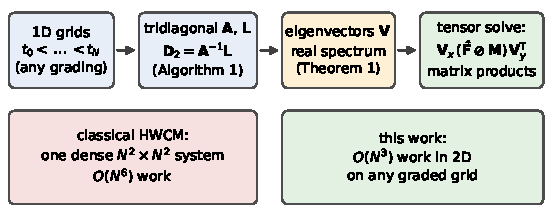
\includegraphics[width=0.95\textwidth]{../figures/panels/pipeline.pdf}
\caption{From the grid to the solution. The one-dimensional operators are assembled from two tridiagonal
matrices; Theorem~\ref{thm:spectrum} guarantees a real eigendecomposition on any grid, and the
multidimensional problem is then solved by dense matrix products instead of one dense system.}\label{fig:pipeline}
\end{figure}

\subsection{Main result: the fast solver always works}
\begin{theorem}[Spectrum on every grid]\label{thm:spectrum}
On every strictly increasing grid, and whether a value or a zero slope is prescribed at each end, the
second-derivative matrix $\mathbf D_2=\mathbf A^{-1}\mathbf L$ has real, distinct and nonpositive eigenvalues. It therefore has a
real eigenvector matrix $\mathbf V$, and fast diagonalization is well defined.
\end{theorem}

In plain terms: whatever grid the user or the refinement algorithm produces, the fast solver of
Section~\ref{sec:tensor} can be used, without complex arithmetic and without restrictions such as a bounded
ratio between neighbouring cells. On uniform grids $\mathbf D_2$ is symmetric, and the result is easy. On graded
grids $\mathbf D_2$ is not symmetric, and the proof (Result~2 in the Supplementary Material) uses the theory of
oscillation matrices, developed by Gantmacher and Krein for vibrating mechanical
systems~\cite{gantmacher2002oscillation}. Fig.~\ref{fig:spectrum} illustrates the result on a grid whose
cells differ in size by three orders of magnitude in random order. The theorem says that the solver is
\emph{defined}; whether it is also \emph{accurate} in floating-point arithmetic is checked separately in
Section~\ref{sec:robust}.

\begin{figure}[t]\centering
\begin{tabular}{@{}cc@{}}
\begin{tabular}[t]{@{}c@{}}\raisebox{-\height}{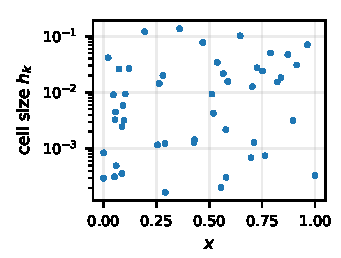
\includegraphics{../figures/panels/spec_grid.pdf}}\end{tabular} &
\begin{tabular}[t]{@{}c@{}}\raisebox{-\height}{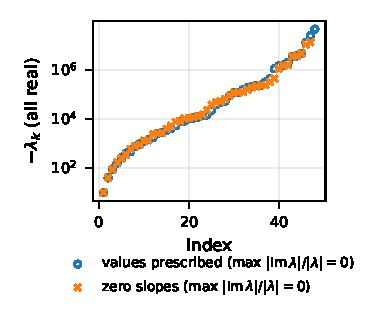
\includegraphics{../figures/panels/spec_eigs.pdf}}\end{tabular}\\
\small (a) & \small (b)\\
\end{tabular}
\caption{Theorem~\ref{thm:spectrum} on a strongly non-uniform grid ($N=48$). (a) Cell sizes, spanning three
orders of magnitude in random order. (b) Eigenvalues of $\mathbf D_2$ for both types of end condition: all are
real (to machine precision), distinct and nonpositive.}\label{fig:spectrum}
\end{figure}

\subsection{Uniform grids: cosine transforms, fourth order and mass conservation}
On a uniform grid, $\mathbf D_2$ is symmetric and is diagonalized by the discrete sine transform (prescribed
values) or cosine transform (zero slopes), so the eigenvectors need not be stored. The corrected operator
\begin{equation}\label{eq:D24}
\mathbf D_2^{(4)}=\mathbf D_2+\tfrac{h^2}{24}\mathbf D_2^2
\end{equation}
has the same eigenvectors and is fourth-order accurate for zero-flux and periodic problems; with general
prescribed values, the order remains two. The correction costs nothing, because in the transform domain it
only changes the eigenvalues. Plain HWCM has half the error constant of the three-point difference, so it
is about twice as accurate on the same grid. Finally, with zero slopes at both ends the weighted sum
$\sum_kh_kU_k$ is conserved exactly by $\mathbf D_2$ on any grid, which gives exact mass conservation for the
Cahn--Hilliard equation. Formal statements and proofs of these properties are Results~3 and~4 of the
Supplementary Material.

%==========================================================================
\section{Fast solvers in two and three dimensions}\label{sec:tensor}
%==========================================================================
On a rectangle, the unknowns form a matrix $\mathbf U=(U_{ij})$, and the one-dimensional operators act along
the grid lines: $\mathbf U_{xx}=\mathbf D_2^x\mathbf U$ and $\mathbf U_{yy}=\mathbf U(\mathbf D_2^y)^{\mathsf T}$, plus boundary terms. An equation such as
$\alpha u_{xx}+\beta u_{yy}+\gamma u=f$ becomes a Sylvester matrix equation. With the eigendecompositions
$\mathbf D_2^x=\mathbf V_x\boldsymbol\Lambda_x\mathbf V_x^{-1}$ and $\mathbf D_2^y=\mathbf V_y\boldsymbol\Lambda_y\mathbf V_y^{-1}$, which exist by Theorem~\ref{thm:spectrum},
its solution is
\begin{equation}\label{eq:fdm}
\mathbf U=\mathbf V_x\Big[\big(\mathbf V_x^{-1}\tilde{\mathbf F}\mathbf V_y^{-\mathsf T}\big)\oslash\mathbf M\Big]\mathbf V_y^{\mathsf T},
\qquad M_{ij}=\alpha\lambda^x_i+\beta\lambda^y_j+\gamma,
\end{equation}
where $\tilde{\mathbf F}$ is the right-hand side including the boundary terms, $\lambda^x_i$ and $\lambda^y_j$
are the eigenvalues, and $\oslash$ denotes entrywise division. This takes four dense matrix products after a one-time
eigendecomposition. In three dimensions the cost is $O(N^4)$, and on uniform grids fast cosine
transforms reduce it to $O(N^d\log N)$. All operations are dense matrix products, fast transforms or
pointwise operations. The code takes the array library (NumPy or CuPy) as a parameter, so the same code
runs on CPUs and GPUs.

%==========================================================================
\section{Phase-field solvers}\label{sec:pf}
%==========================================================================
We solve the Allen--Cahn (AC) and Cahn--Hilliard (CH) equations with zero-flux boundaries,
$u_t=-\mathcal G\mu$, $\mu=-\varepsilon^2\Delta u+u^3-u$, with $\mathcal G$ the identity for AC and $\mathcal G=-\Delta$
for CH. The parameter $\varepsilon$ sets the interface thickness. Across an equilibrium interface
$u\approx\tanh(d/\sqrt2\varepsilon)$, where $d$ is the distance to the interface. In time we use the
stabilized SAV-BDF2 scheme~\cite{shen2018scalar} (\ref{app:sav}). It treats the nonlinear term explicitly
through a scalar auxiliary variable, so each step needs only one forward and one inverse transform and a
division in the transform domain. On a uniform grid it is uniquely solvable for every time step, conserves
the discrete mass exactly, and a modified energy never increases. The scheme works in three dimensions as
well; a three-dimensional accuracy test is reported in Table~S18.

This guarantee concerns a \emph{modified} energy. That the physical energy decreases, that $u$ stays
bounded, and that interfaces move correctly are properties we observe but do not prove, and for thin
interfaces they need stabilization: with $S=0$, a computation with $\varepsilon=0.0015$ produced values of
$|u|$ around 30 to 70, whereas $S=4$ kept $|u|\le1.04$ (Table~S25). In a systematic study
(Table~S17), $S\approx1$ to 2 was best for time steps up to $\varepsilon^2$, and 2 to 4 for larger steps.
Steps much larger than $\varepsilon^2$ give wrong interface motion even with stabilization.

%==========================================================================
\section{Elastostatics}\label{sec:elast}
%==========================================================================
For plane strain we enforce the Navier equations at the cell midpoints. Because $u$ and $v$ are coupled,
we use GMRES, preconditioned by two decoupled fast-diagonalization solves per iteration, one for each
displacement component. For compressible materials the number of iterations does not grow with the grid;
as Poisson's ratio approaches one half it grows strongly (Tables~S1 and~S2), so the solver is intended for
compressible materials. On a traction edge, the edge displacements become unknowns, and
$\boldsymbol\sigma\mathbf n=\mathbf t$ is enforced at the edge midpoints. The normal derivatives come from
the end slopes of Algorithm~1, and the tangential derivatives from $\mathbf D_1$ along the edge. Where two traction
edges meet, the two normal stresses are prescribed. Unlike quadratic isogeometric collocation, where
pointwise traction conditions can lose accuracy and an ``enhanced'' boundary equation is
recommended~\cite{delorenzis2015isogeometric}, plain collocation stays second-order accurate here. With tractions on two adjacent edges and $\nu=0.3$,
the relative $H^1$ error decreases from $4.3\times10^{-3}$ at $N=16$ to $1.7\times10^{-5}$ at
$N=256$ (observed rate 2.00), and the largest displacement error on the traction edges is
$1.8\times10^{-5}$; on a geometric grid graded toward the traction edge with cell-size ratio up to
85, the rate is again two (Tables~S9 and~S10). In the preconditioner, a traction edge is treated as a zero-slope end,
which is again covered by Theorem~\ref{thm:spectrum}.

For adaptivity we use the Haar coefficients directly. The finest-level Haar coefficient of $u''$ is
proportional to the jump of $u''$ between neighbouring cells, and this jump measures the local error of
the gradient. For each cell of the $x$-direction grid we compute
\begin{equation}\label{eq:indicator}
\eta^x_i{}^2=h^x_i{}^3\sum_jh^y_j\,\tfrac12\Big([\![u_{xx}]\!]_{i-\frac12,j}^2+[\![u_{xx}]\!]_{i+\frac12,j}^2\Big),
\end{equation}
summed over both displacement components, and similarly in $y$. Algorithm~3 marks and bisects the cells
with the largest indicators. The indicator is heuristic, in the sense that no error bound is proved for it,
but in all our tests it followed the true error closely.

\begin{algorithm}[t]\small\hrule\smallskip
\noindent\textbf{Algorithm 3: adaptive elastostatics} (\texttt{ihaar/elasticity\_bc.py}).
\step{1} Start from a uniform tensor grid, for example $8\times8$ cells.
\step{2} Build the one-dimensional operators (Algorithm~1) and the preconditioner factorizations, and solve with right-preconditioned GMRES (relative tolerance $10^{-10}$, restart length 60 to 80).
\step{3} Compute the indicators $\eta^x_i$ and $\eta^y_j$ from~\eqref{eq:indicator}.
\step{4} Mark the smallest set of one-dimensional cells, in both directions together, that carries a fraction $\theta=0.6$ of $\sum\eta^2$ (D\"orfler marking~\cite{dorfler1996convergent}), and bisect them.
\step{5} Bisect further until neighbouring cells differ in size by at most a factor of two, and return to Step~2.
\smallskip\hrule
\end{algorithm}

%==========================================================================
\section{Results}\label{sec:results}
%==========================================================================
All computations ran in double precision on the system described in Table~S20; absolute
timings depend on this hardware and software. Every number is produced by the scripts of the repository,
and the tables are generated from the stored results.

\subsection{Verification and cost}\label{sec:verify}
Fig.~\ref{fig:verify}(a) shows the maximum nodal error for $-\Delta u=f$ with prescribed values and
$u=e^x\sin\pi y+x^2y$, on uniform and on Chebyshev-graded grids, and for $u-\Delta u=f$ with zero slopes
and $u=\cos\pi x\cos2\pi y+0.3\cos3\pi x$. The plain operator converges at second order on both grid
families, and the corrected operator at fourth order. Second-order convergence was also observed for
smooth elastostatic solutions with prescribed displacements and with tractions, in three dimensions, and
for the Cahn--Hilliard equation, where the corrected operator gives fourth order (Tables~S8, S9, S18,
S13 and~S21). Fig.~\ref{fig:verify}(b) shows the practical gain over classical HWCM: on our hardware the
dense HWCM solve takes 0.7~s at $64\times64$ cells and is infeasible beyond that, whereas the
cosine-transform solver handles $10^6$ unknowns in 0.04~s, and fast diagonalization on a graded
grid is only a few times slower.

\begin{figure}[t]\centering
\begin{tabular}{@{}cc@{}}
\begin{tabular}[t]{@{}c@{}}\raisebox{-\height}{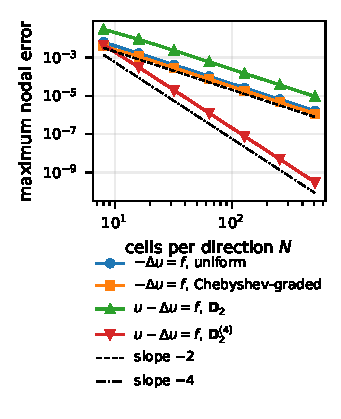
\includegraphics{../figures/panels/verification.pdf}}\end{tabular} & \begin{tabular}[t]{@{}c@{}}\raisebox{-\height}{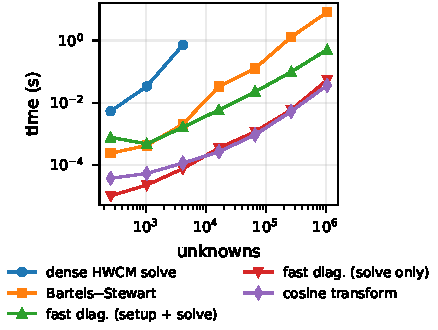
\includegraphics{../figures/panels/cost.pdf}}\end{tabular}\\
\small (a) & \small (b)\\
\end{tabular}\par\smallskip
\caption{(a) Maximum nodal error versus cells per direction for two model problems. (b) Wall time of one solve with $N^2$ unknowns for the classical dense HWCM system, the Bartels--Stewart algorithm, fast diagonalization and the cosine transform (data in Tables~S21 and~S23).}\label{fig:verify}
\end{figure}

\subsection{Reliability of the fast solver}\label{sec:robust}
Theorem~\ref{thm:spectrum} guarantees that fast diagonalization is defined on every grid, but not that
its result is accurate in floating-point arithmetic. We therefore compared it with the backward-stable
Bartels--Stewart algorithm~\cite{bartels1972solution} on 8760 random graded grids and on deliberately
adversarial grids, with cell-size ratios up to $10^{12}$ (Tables~S4, S15 and~S22). The
eigenvalues were real in every case, and fast diagonalization was as accurate as Bartels--Stewart up to
round-off. Only on the most extreme grids did the two solutions differ, and there the discrete problem
itself is so ill conditioned that no solver can be accurate in double precision. The code checks every
solve at the cost of two matrix products and switches to Bartels--Stewart if needed, which never
happened in our computations; it also warns when the problem is ill conditioned. On all grids produced by
the refinement algorithm the eigenvector condition number stayed below 25.

\subsection{Elastostatics: a crack-like corner and a comparison with finite elements}\label{sec:q2}
We use the exact Mode-I field of a re-entrant corner of opening $3\pi/2$~\cite{williams1952stress}, whose
displacements behave like $r^{0.544}$ near the corner. The square is placed so that its top edge lies on a
traction-free face and the singular point is at the end of that face. This is the local situation at the
re-entrant corner of the L-shaped benchmark. Uniform grids converge slowly, like
$\mathrm{DOF}^{-0.27}$, and reach a relative $H^1$ error of $1.9\times10^{-2}$ with 132\,000 unknowns.
Automatic refinement reaches $1.2\times10^{-4}$ with 149\,000 unknowns, at the optimal rate
$\mathrm{DOF}^{-1}$, with 15 to 20 GMRES iterations for $\nu=0.3$ (Fig.~\ref{fig:trac}). The grading is found
automatically. A second test, with prescribed displacements on all edges, behaves in the same way
(Table~S11). Further tests with four corner openings (down to a near-crack), two singular corners, and a
boundary layer all gave rates between $-0.95$ and $-1.05$, close to those obtained by refining according to
the true error (Fig.~\ref{fig:adapt} and Table~S16). These rates are observations, not a general theorem. Because
tensor refinement extends refinement lines across the domain, the grids contain about four times more
cells than an ideal local refinement would, but this does not affect the convergence rate.
Section~\ref{sec:local} shows how this factor can be removed.

\begin{figure}[t]\centering
\begin{tabular}{@{}cc@{}}
\begin{tabular}[t]{@{}c@{}}\raisebox{-\height}{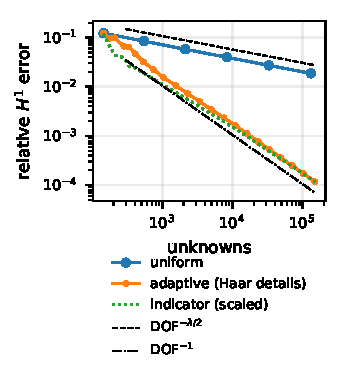
\includegraphics{../figures/panels/trac_error.pdf}}\end{tabular} & \begin{tabular}[t]{@{}c@{}}\raisebox{-\height}{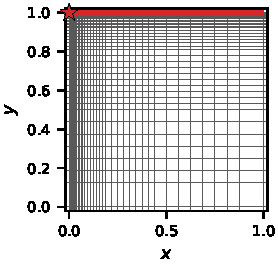
\includegraphics{../figures/panels/trac_grid.pdf}}\end{tabular}\\
\small (a) & \small (b)\\
\end{tabular}\par\smallskip
\begin{tabular}{@{}c@{}}
\begin{tabular}[t]{@{}c@{}}\raisebox{-\height}{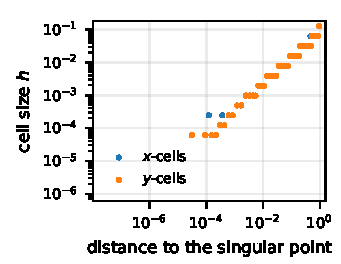
\includegraphics{../figures/panels/trac_cellsize.pdf}}\end{tabular}\\
\small (c)\\
\end{tabular}\par\smallskip
\caption{Corner singularity at the end of a traction-free face ($\nu=0.3$). (a) Relative $H^1$ error versus number of unknowns for uniform and automatic refinement, with the scaled indicator. (b) Grid generated after 12 refinement cycles; the red edge is the traction-free face and the star marks the singular point. (c) Cell size versus distance to the singular point on the grid of (b).}\label{fig:trac}
\end{figure}

Fig.~\ref{fig:elfields} shows the computed stress
field on the adapted grid of Fig.~\ref{fig:trac}(b). The von Mises stress follows the exact singular field,
which grows like $r^{-0.456}$, over more than four decades of distance to the singular point, down to the
size of the smallest cell.

\begin{figure}[t]\centering
\begin{tabular}{@{}cc@{}}
\begin{tabular}[t]{@{}c@{}}\raisebox{-\height}{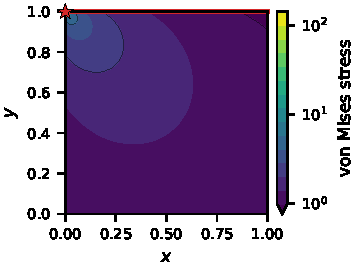
\includegraphics{../figures/panels/el_vm.pdf}}\end{tabular} & \begin{tabular}[t]{@{}c@{}}\raisebox{-\height}{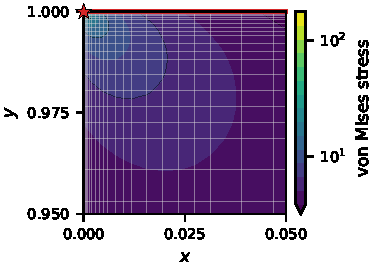
\includegraphics{../figures/panels/el_vm_zoom.pdf}}\end{tabular}\\
\small (a) & \small (b)\\
\end{tabular}\par\smallskip
\begin{tabular}{@{}c@{}}
\begin{tabular}[t]{@{}c@{}}\raisebox{-\height}{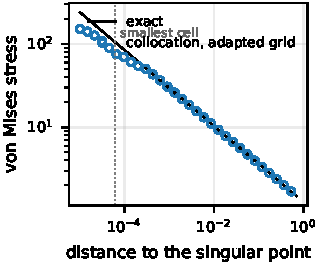
\includegraphics{../figures/panels/el_vm_line.pdf}}\end{tabular}\\
\small (c)\\
\end{tabular}\par\smallskip
\caption{Stress field for the corner singularity of Fig.~\ref{fig:trac} ($\nu=0.3$), computed on the grid of Fig.~\ref{fig:trac}(b). (a) von Mises stress on the whole domain (logarithmic colour scale). (b) Zoom at the singular point, with the grid lines. (c) von Mises stress along the line at $45^\circ$ into the body versus distance to the singular point, compared with the exact field.}\label{fig:elfields}
\end{figure}

\begin{figure}[t]\centering
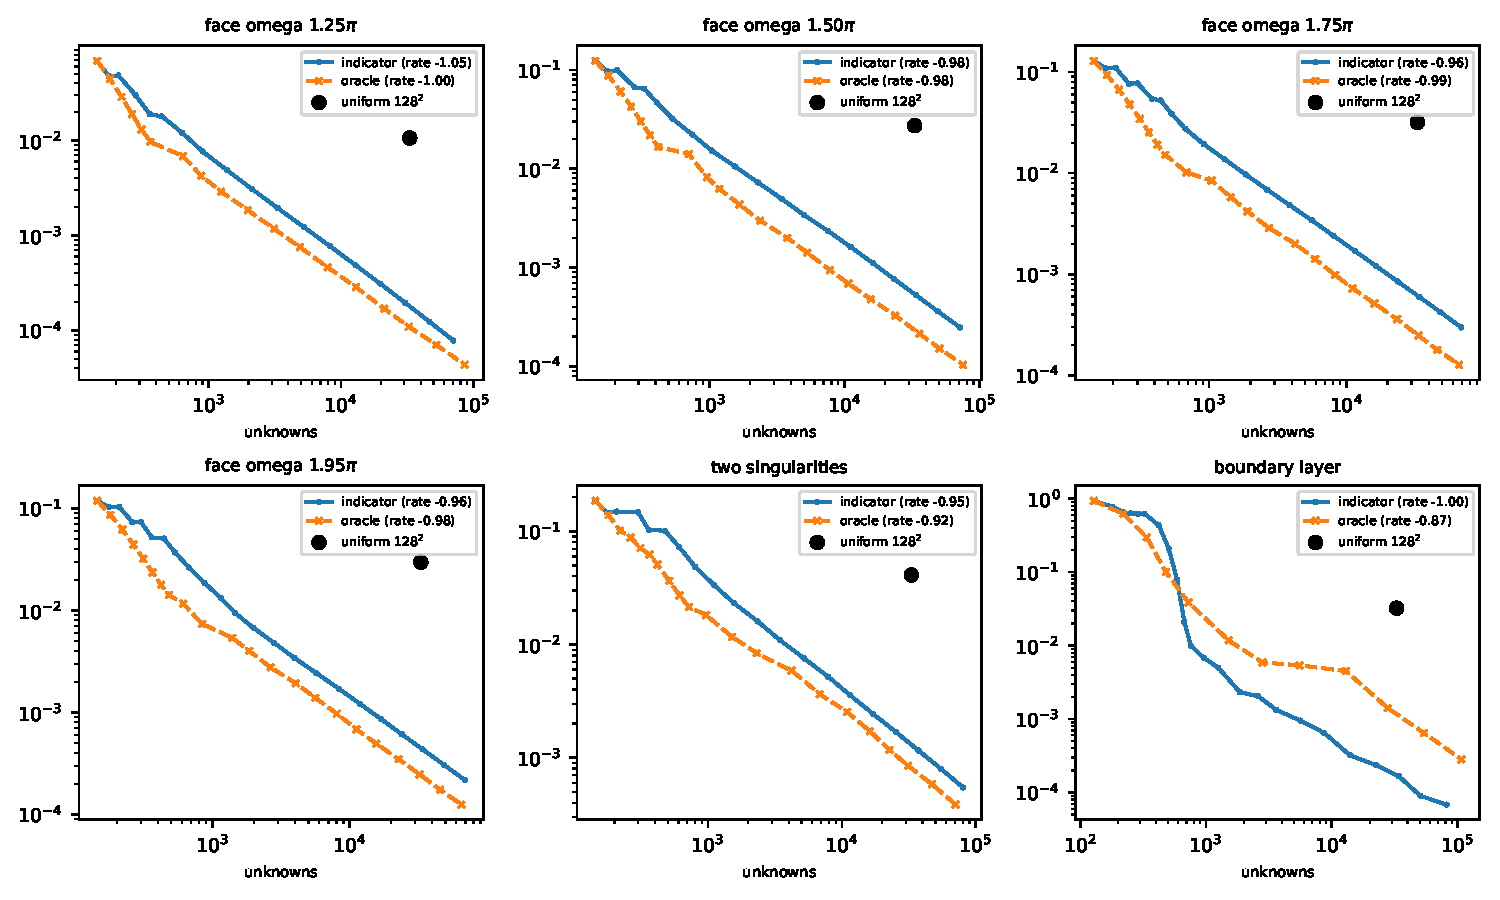
\includegraphics[width=\textwidth]{../figures/adaptivity_cases.pdf}
\caption{Automatic refinement for six further configurations: corners of opening $1.25\pi$ to $1.95\pi$ at
the end of a traction-free face, two singular corners, and a boundary layer. Relative $H^1$ error versus
unknowns for the Haar-detail indicator and for refinement by the true error (oracle), with fitted rates
(data in Table~S16).}\label{fig:adapt}
\end{figure}

To put these numbers in context, we solved the same problem with biquadratic ($Q_2$) finite elements on
exactly the same grids, with the same type of solver: conjugate gradients preconditioned by fast
diagonalization (Table~\ref{tab:q2} and Fig.~\ref{fig:q2}). On a given grid, $Q_2$ is about 1.3 times more
accurate, but it has four times as many unknowns. In this benchmark, at equal accuracy, the collocation method needed about a quarter of the unknowns of $Q_2$. In our implementation and on our hardware this translated into about 3.6 times less end-to-end time
including assembly (about 1.1 times without it) and about 30\% less memory. These time and memory factors depend on implementation and
hardware; the factor in unknowns does not. A sparse direct solver was about 70 times slower than conjugate gradients with the
fast-diagonalization preconditioner (11.2~s at 193\,980 unknowns), so much of the speed-up often reported for structured methods comes from the
solver. \todo{AMG baseline pending: \texttt{pip install pyamg}, then run E13 (see README).}


\begin{table}[t]\centering\small
\caption{Collocation versus $Q_2$ finite elements on identical grids (every third refinement cycle).
Memory counts operators, factorizations and Krylov vectors.}\label{tab:q2}
\textit{(a) IHWC collocation: GMRES with the FDM preconditioner}\\[2pt]
\begin{tabular}{rr c ccc}
\toprule
cycle & unknowns & $e_{H^1}$ & setup (s) & solve (s) & MB\\
\midrule
0 & 144 & $1.23{\times}10^{-1}$ & 0.00 & 0.00 & 0.3\\
3 & 280 & $6.68{\times}10^{-2}$ & 0.00 & 0.01 & 0.4\\
6 & 532 & $3.22{\times}10^{-2}$ & 0.00 & 0.01 & 0.6\\
9 & 1550 & $1.05{\times}10^{-2}$ & 0.00 & 0.01 & 1.3\\
12 & 4982 & $3.42{\times}10^{-3}$ & 0.01 & 0.01 & 3.9\\
15 & 16182 & $1.11{\times}10^{-3}$ & 0.02 & 0.04 & 12.3\\
18 & 48960 & $3.59{\times}10^{-4}$ & 0.06 & 0.13 & 37.0\\
21 & 149008 & $1.17{\times}10^{-4}$ & 0.21 & 0.48 & 112.3\\
22 & 215644 & $8.03{\times}10^{-5}$ & 0.44 & 0.78 & 162.5\\
\bottomrule
\end{tabular}

\medskip
\textit{(b) $Q_2$ finite elements on the same grids, same cycles (rows) as in (a): CG with the FDM preconditioner, and sparse direct solve}\\[2pt]
\begin{tabular}{r c cccc}
\toprule
unknowns & $e_{H^1}$ & asm.\ (s) & CG (s) & MB & direct (s)\\
\midrule
480 & $7.22{\times}10^{-2}$ & 0.00 & 0.00 & 0.2 & 0.00\\
988 & $5.39{\times}10^{-2}$ & 0.01 & 0.00 & 0.3 & 0.00\\
1944 & $2.61{\times}10^{-2}$ & 0.01 & 0.00 & 0.7 & 0.02\\
5880 & $8.43{\times}10^{-3}$ & 0.02 & 0.01 & 2.0 & 0.06\\
19344 & $2.73{\times}10^{-3}$ & 0.04 & 0.03 & 6.8 & 0.51\\
63664 & $8.80{\times}10^{-4}$ & 0.13 & 0.09 & 22.7 & 3.08\\
193980 & $2.84{\times}10^{-4}$ & 0.39 & 0.32 & 69.4 & 20.49\\
592780 & $9.21{\times}10^{-5}$ & 1.54 & 1.19 & 212.6 & --\\
858676 & $6.33{\times}10^{-5}$ & 2.10 & 2.18 & 308.2 & --\\
\bottomrule
\end{tabular}

\end{table}
\begin{figure}[t]\centering
\begin{tabular}{@{}cc@{}}
\begin{tabular}[t]{@{}c@{}}\raisebox{-\height}{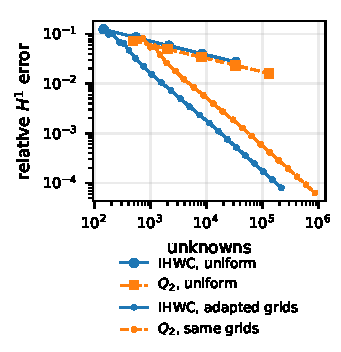
\includegraphics{../figures/panels/q2_error.pdf}}\end{tabular} & \begin{tabular}[t]{@{}c@{}}\raisebox{-\height}{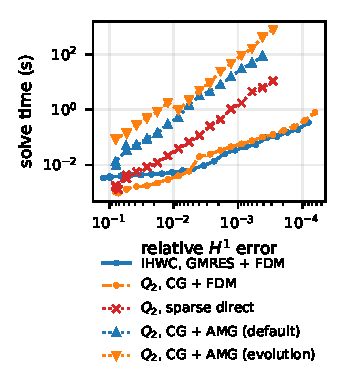
\includegraphics{../figures/panels/q2_time.pdf}}\end{tabular}\\
\small (a) & \small (b)\\
\end{tabular}\par\smallskip
\caption{Collocation (IHWC) versus $Q_2$ finite elements on identical grids. (a) Error versus number of unknowns. (b) Solve time versus error for IHWC and for $Q_2$ with CG and the fast-diagonalization preconditioner, a sparse direct solver, and CG with algebraic multigrid (converged solves only).}\label{fig:q2}
\end{figure}

\subsection{Local refinement with composite patches}\label{sec:local}
Tensor refinement extends refinement lines across the domain. True local refinement is possible without
giving up the fast solver, by covering the singular region with nested rectangular patches
$P_k=(0,2^{-k})^2$, $k=0,\dots,L$, each with its own uniform $n\times n$ grid (Fig.~\ref{fig:local}(a)).
Theorem~\ref{thm:spectrum} applies to every patch, so each patch is solved by fast diagonalization. A patch
takes the values on its two interior edges from the spline of the next coarser patch. Conversely, in a
region at least three coarse cells inside the finer patch, the coarser patch replaces its collocation
equations, written in the tridiagonal form of the identity~\eqref{eq:identity}, by those of the
interpolated fine solution, so that it sees the fine solution there. The coupled problem is solved by
sweeping over the patches from coarse to fine and back, and each point is represented by the finest patch
that contains it (\texttt{ihaar/composite.py}).

We tested this on the Laplace equation on the unit square with $u=r^{2/3}\sin(2\theta/3)$, whose gradient
is singular at a corner, against the tensor grid that has the same local resolution, namely the union of
the patch grids (Fig.~\ref{fig:local}(b) and Table~S27). The sweeps converged to round-off in 4 to 5
sweeps in every case, and the composite solution had the accuracy of the tensor grid. The number of unknowns
grows linearly with the number of levels instead of quadratically. With balanced refinement, the fitted rate
improves from $-0.79$ to $-0.89$ (the optimal rate is $-1$ up to a logarithmic factor), and at the
finest level the patches need 3.8 times fewer unknowns and 3.9 times less time.
This is a demonstration for a scalar problem with a point singularity. The extension to elasticity, where
each patch solve is itself a preconditioned GMRES iteration, and to singularities along lines remains to be
done.

\begin{figure}[t]\centering
\begin{tabular}{@{}cc@{}}
\begin{tabular}[t]{@{}c@{}}\raisebox{-\height}{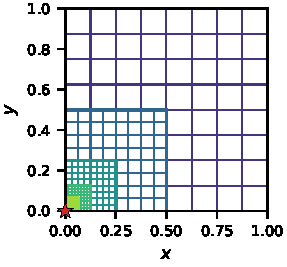
\includegraphics{../figures/panels/local_patches.pdf}}\end{tabular} & \begin{tabular}[t]{@{}c@{}}\raisebox{-\height}{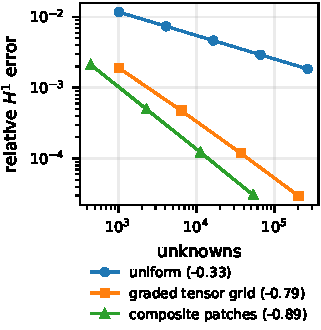
\includegraphics{../figures/panels/local_error.pdf}}\end{tabular}\\
\small (a) & \small (b)\\
\end{tabular}\par\smallskip
\caption{Local refinement by composite patches (Laplace equation, corner singularity at the star). (a) Nested patches, here with $L=4$ levels of $8\times8$ cells. (b) Relative $H^1$ error versus unknowns for uniform grids, the tensor grid with the same local resolution, and the composite patches, with fitted rates (balanced refinement, $L=2\log_2n$).}\label{fig:local}
\end{figure}

\subsection{Phase field: how many nodes does an interface need?}\label{sec:sharp}
Across an interface, $u$ goes from $-0.76$ to $0.76$ over a distance of $2\sqrt2\varepsilon$, so we measure
resolution in nodes per $\sqrt2\varepsilon$. For a planar interface solved exactly on discrete grids
(Fig.~\ref{fig:res}), plain HWCM is about twice as accurate as the standard three-point difference at every
resolution. The fourth-order operator pays off from about 1.5 nodes per $\sqrt2\varepsilon$. At 3.6 nodes it
is 25 times more accurate than finite differences, and at 7.2 nodes 110 times.

\begin{figure}[t]\centering
\begin{tabular}{@{}c@{}}
\begin{tabular}[t]{@{}c@{}}\raisebox{-\height}{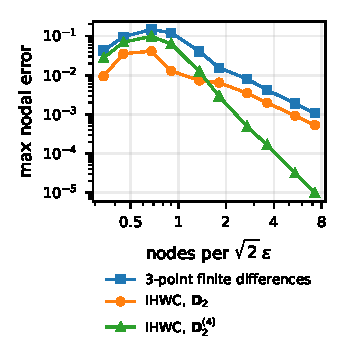
\includegraphics{../figures/panels/resolution.pdf}}\end{tabular}\\
\end{tabular}\par\smallskip
\caption{Planar interface ($\varepsilon=0.01$): maximum nodal error versus nodes per $\sqrt2\varepsilon$ (data in Table~S5).}\label{fig:res}
\end{figure}

For a shrinking circle under Allen--Cahn dynamics
($\varepsilon=0.02$), sharp-interface theory predicts that $R^2$ decreases linearly at the rate $2\varepsilon^2$.
The computed rate on $256^2$ deviates from it by 0.4\%, and the energy decreases
monotonically on all grids (Fig.~\ref{fig:ac} and Table~S12).

\begin{figure}[t]\centering
\begin{tabular}{@{}cc@{}}
\begin{tabular}[t]{@{}c@{}}\raisebox{-\height}{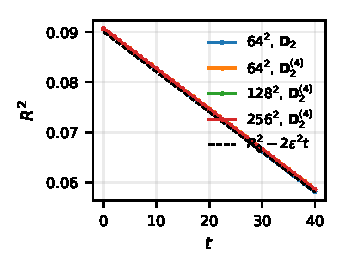
\includegraphics{../figures/panels/ac_radius.pdf}}\end{tabular} & \begin{tabular}[t]{@{}c@{}}\raisebox{-\height}{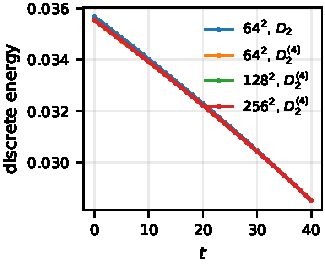
\includegraphics{../figures/panels/ac_energy.pdf}}\end{tabular}\\
\small (a) & \small (b)\\
\end{tabular}\par\smallskip
\caption{Allen--Cahn shrinking circle ($\varepsilon=0.02$, $\Delta t=0.05$). (a) Squared radius versus time, with the sharp-interface law. (b) Discrete energy.}\label{fig:ac}
\end{figure}

For the Allen--Cahn six-fold star with $\varepsilon=0.004$, evolving under curvature flow, a $1024^2$
computation serves as the reference (Fig.~\ref{fig:star} and Table~\ref{tab:star}). On $256^2$, which gives
only 1.45 nodes per $\sqrt2\varepsilon$, the sharp tips move too slowly with $\mathbf D_2$, while $\mathbf D_2^{(4)}$ follows
the reference. $\mathbf D_2^{(4)}$ on $256^2$ is as accurate in area as $\mathbf D_2$ on $512^2$, with a quarter of the
unknowns, and on $512^2$ it is 16 times more accurate than $\mathbf D_2$.

\begin{figure}[t]\centering
\begin{tabular}{@{}cc@{}}
\begin{tabular}[t]{@{}c@{}}\raisebox{-\height}{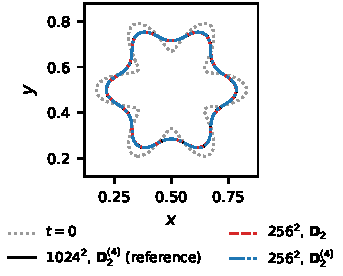
\includegraphics{../figures/panels/star_levelsets.pdf}}\end{tabular} & \begin{tabular}[t]{@{}c@{}}\raisebox{-\height}{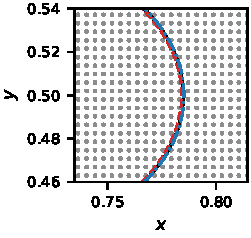
\includegraphics{../figures/panels/star_zoom.pdf}}\end{tabular}\\
\small (a) & \small (b)\\
\end{tabular}\par\smallskip
\begin{tabular}{@{}c@{}}
\begin{tabular}[t]{@{}c@{}}\raisebox{-\height}{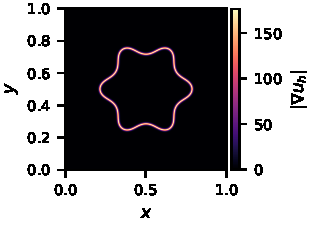
\includegraphics{../figures/panels/star_gradient.pdf}}\end{tabular}\\
\small (c)\\
\end{tabular}\par\smallskip
\caption{Allen--Cahn star, $\varepsilon=0.004$, at $t=120$. (a) Zero level sets of the reference and of the $256^2$ solutions, and the initial interface. (b) Zoom at a tip, with the $256^2$ grid nodes. (c) Gradient magnitude of the reference solution.}\label{fig:star}
\end{figure}
\begin{table}[t]\centering\small
\caption{Allen--Cahn star ($\varepsilon=0.004$): maximum nodal error and area error against the $1024^2$
reference, and cost per step.}\label{tab:star}
\begin{tabular}{ll ccc}
\toprule
grid & operator & max nodal error & area error & ms per step\\
\midrule
$256^2$ & $\mathbf D_2$ & $1.36{\times}10^{-1}$ & $2.43{\times}10^{-4}$ & 1.5\\
$256^2$ & $\mathbf D_2^{(4)}$ & $5.27{\times}10^{-2}$ & $6.07{\times}10^{-5}$ & 1.5\\
$512^2$ & $\mathbf D_2$ & $4.12{\times}10^{-2}$ & $6.88{\times}10^{-5}$ & 9.0\\
$512^2$ & $\mathbf D_2^{(4)}$ & $2.63{\times}10^{-3}$ & $4.23{\times}10^{-6}$ & 9.2\\
$1024^2$ (reference) & $\mathbf D_2^{(4)}$ & -- & -- & 93\\
\bottomrule
\end{tabular}

\end{table}

The most demanding case is Cahn--Hilliard with $\varepsilon=0.0015$ on $1024^2$, which gives 2.2 nodes per
$\sqrt2\varepsilon$; the whole interface spans about four nodes. With stabilized SAV ($S=4$), mass is
conserved to $10^{-17}$, both the modified and the physical energy decrease, $|u|$ stays below 1.03, and the
nodal profile across an interface coincides with the exact $\tanh$ profile. The largest computed gradient,
467, matches the exact value $1/(\sqrt2\varepsilon)=471$ (Fig.~\ref{fig:chsharp} and Table~S24).

\begin{figure}[t]\centering
\begin{tabular}{@{}ccc@{}}
\begin{tabular}[t]{@{}c@{}}\raisebox{-\height}{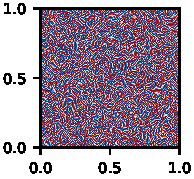
\includegraphics{../figures/panels/ch_snap0.pdf}}\end{tabular} & \begin{tabular}[t]{@{}c@{}}\raisebox{-\height}{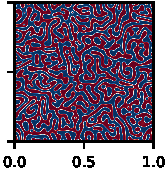
\includegraphics{../figures/panels/ch_snap1.pdf}}\end{tabular} & \begin{tabular}[t]{@{}c@{}}\raisebox{-\height}{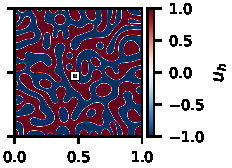
\includegraphics{../figures/panels/ch_snap2.pdf}}\end{tabular}\\
\small (a) & \small (b) & \small (c)\\
\end{tabular}\par\smallskip
\begin{tabular}{@{}cc@{}}
\begin{tabular}[t]{@{}c@{}}\raisebox{-\height}{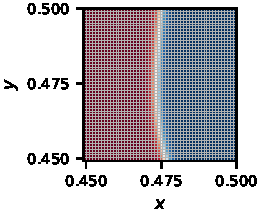
\includegraphics{../figures/panels/ch_zoom.pdf}}\end{tabular} & \begin{tabular}[t]{@{}c@{}}\raisebox{-\height}{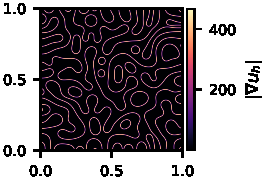
\includegraphics{../figures/panels/ch_gradient.pdf}}\end{tabular}\\
\small (d) & \small (e)\\
\end{tabular}\par\smallskip
\begin{tabular}{@{}cc@{}}
\begin{tabular}[t]{@{}c@{}}\raisebox{-\height}{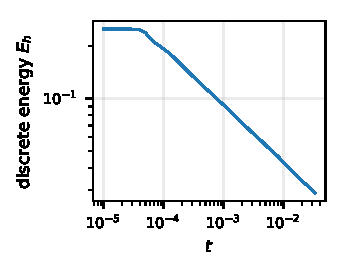
\includegraphics{../figures/panels/ch_energy.pdf}}\end{tabular} & \begin{tabular}[t]{@{}c@{}}\raisebox{-\height}{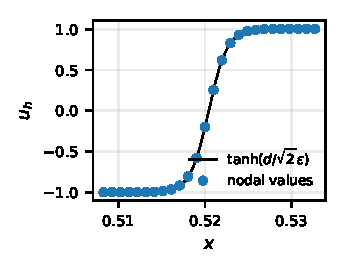
\includegraphics{../figures/panels/ch_profile.pdf}}\end{tabular}\\
\small (f) & \small (g)\\
\end{tabular}\par\smallskip
\caption{Cahn--Hilliard with $\varepsilon=0.0015$ on $1024^2$. (a)--(c) Concentration at $t=0.0003$, $0.0033$ and $0.0333$; the box in (c) marks the region shown in (d). (d) Zoom in which each square is one node. (e) Gradient magnitude at the final time. (f) Discrete energy. (g) Nodal values along a grid line crossing an interface, compared with the $\tanh$ profile.}\label{fig:chsharp}
\end{figure}
Fig.~\ref{fig:surf} shows the final states of the two
thin-interface computations as surfaces. The solution consists of flat plateaus at $u=\pm1$ joined by
walls only a few cells wide. The zooms are plotted at full resolution, one surface facet per node: the
walls are resolved without visible oscillations, and $|u_h|$ exceeds one by at most 2.8\%
for Cahn--Hilliard and only at round-off level
for Allen--Cahn.

\begin{figure}[t]\centering
\begin{tabular}{@{}cc@{}}
\begin{tabular}[t]{@{}c@{}}\raisebox{-\height}{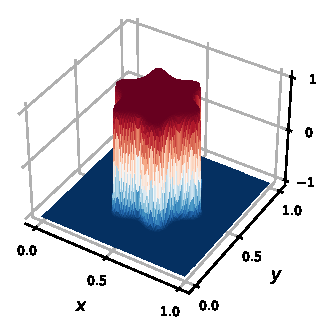
\includegraphics{../figures/panels/surf_star.pdf}}\end{tabular} & \begin{tabular}[t]{@{}c@{}}\raisebox{-\height}{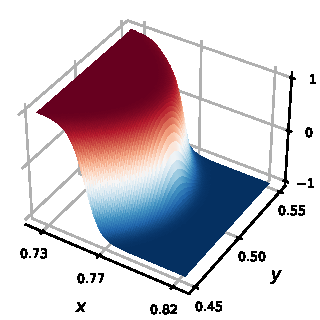
\includegraphics{../figures/panels/surf_star_tip.pdf}}\end{tabular}\\
\small (a) & \small (b)\\
\end{tabular}\par\smallskip
\begin{tabular}{@{}c@{}}
\begin{tabular}[t]{@{}c@{}}\raisebox{-\height}{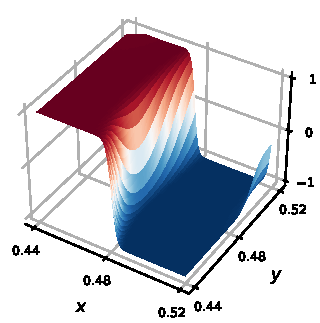
\includegraphics{../figures/panels/surf_ch.pdf}}\end{tabular}\\
\small (c)\\
\end{tabular}\par\smallskip
\caption{Final states as surfaces. (a) Allen--Cahn star at $t=120$ ($1024^2$ reference, every fourth node shown). (b) Zoom at a tip of (a), every node shown. (c) Cahn--Hilliard with $\varepsilon=0.0015$ on $1024^2$ at the final time, window $[0.44,0.52]^2$ (containing the zoom of Fig.~\ref{fig:chsharp}(d)), every node shown.}\label{fig:surf}
\end{figure}

\subsection{When not to use the method}\label{sec:compare}
Because every uniform-grid operator considered here is diagonalized by the same cosine transform, we
could compare five of them within the identical solver: the three-point difference, $\mathbf D_2$, $\mathbf D_2^{(4)}$,
the classical compact (Pad\'e) scheme, and the cosine pseudo-spectral method (Fig.~\ref{fig:compare} and
Table~S14). Plain HWCM beats the three-point difference by a factor of two, and the compact scheme is about
1.4 times more accurate than $\mathbf D_2^{(4)}$. For smooth problems on uniform boxes with zero-flux or periodic
conditions, however, the pseudo-spectral method is far more accurate than all others. For such problems we
recommend pseudo-spectral methods. The strength of the present method lies in graded and adaptive grids,
prescribed values and tractions, and singular solutions. The elastostatic formulation is also not robust
as Poisson's ratio approaches one half (Tables~S1 and~S2).

\begin{figure}[t]\centering
\begin{tabular}{@{}c@{}}
\begin{tabular}[t]{@{}c@{}}\raisebox{-\height}{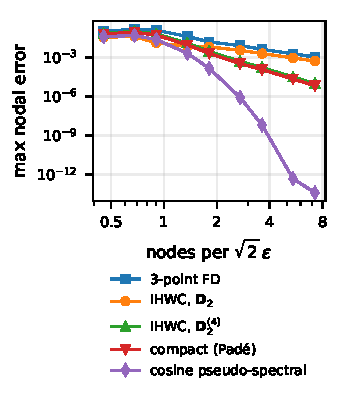
\includegraphics{../figures/panels/scheme_comparison.pdf}}\end{tabular}\\
\end{tabular}\par\smallskip
\caption{Planar interface: maximum nodal error versus resolution for five operators.}\label{fig:compare}
\end{figure}

\subsection{Performance}
A phase-field time step costs $O(N^d\log N)$ operations with fast cosine transforms. On the CPU of Table~S20 this amounted to between $10^{7}$ and $5\times10^{7}$ unknowns per second (Table~S26). Absolute timings
depend on the hardware; the complexity does not. GPU timings were measured on an NVIDIA GeForce RTX 3050 Ti Laptop GPU (CUDA 13.2, CuPy 14.2.0); times are per step after warm-up, with device synchronization.


%==========================================================================
\section{Practical guidelines}\label{sec:guide}
%==========================================================================
Table~\ref{tab:guide} summarizes the choices that worked in our computations.

\begin{table}[t]\centering\small
\caption{Practical recommendations.}\label{tab:guide}
\begin{tabular}{>{\raggedright\arraybackslash}p{0.22\textwidth}>{\raggedright\arraybackslash}p{0.72\textwidth}}
\toprule
Decision & Recommendation\\
\midrule
Plain or corrected operator & Use $\mathbf D_2^{(4)}$ for zero-flux or periodic problems, since it costs nothing extra. With general prescribed values, use $\mathbf D_2$, because the correction does not raise the order there.\\
When not to use IHWC & For smooth or phase-field problems on uniform boxes with zero-flux or periodic conditions, a cosine pseudo-spectral operator is far more accurate at the same cost (Section~\ref{sec:compare}).\\
Interface resolution & Use at least 1.5 nodes per $\sqrt2\varepsilon$ with $\mathbf D_2^{(4)}$. Expect a nodal error of about $10^{-3}$ at 2 to 3 nodes, and about $10^{-4}$ at 3.5 nodes (Table~S5).\\
Time stepping (AC, CH) & Use SAV-BDF2 with the smallest stabilization that keeps $\xi=r/\sqrt{E_{1,h}+C}$ near one: $S\approx1$ to 2 for $\Delta t\lesssim\varepsilon^2$, and 2 to 4 for larger steps (Table~S17). Keep $\Delta t$ of order $\varepsilon^2$ when the coarsening dynamics matter, and verify by halving $\Delta t$; $\xi\approx1$ alone does not guarantee accuracy.\\
Solver & On uniform grids, use cosine or sine transforms. On graded grids, use fast diagonalization (well defined by Theorem~\ref{thm:spectrum}) with the built-in check and Bartels--Stewart fallback, and heed the ill-conditioning warning. For coupled systems such as elasticity, use GMRES with the block preconditioner.\\
Adaptivity at singularities & Use the Haar-detail indicator with D\"orfler parameter $\theta\approx0.6$, a neighbour ratio of at most two, and an initial grid of $8\times8$ cells.\\
Traction conditions & Collocate tractions plainly at edge midpoints, without enhancement, and use the two normal-stress conditions at traction--traction corners.\\
Near incompressibility & Avoid $\nu>0.45$ with the present formulation (Tables~S1 and~S2).\\
\bottomrule
\end{tabular}
\end{table}

%==========================================================================
\section{Limitations}\label{sec:limits}
%==========================================================================
The fast solvers require rectangular domains; the full L-shaped domain and curved boundaries need
multi-patch coupling or geometry maps. Line refinement is anisotropic but not local, which costs a
constant factor of about four in cells at point singularities; composite patches remove this factor, but
so far they have been tested only for the Laplace equation (Section~\ref{sec:local}). Proved results and observations should be
distinguished. Proved are the three-term identity, the real spectrum on every grid, the fourth-order
correction and the symmetric structure on uniform grids, exact mass conservation, and the decay of the
modified energy on uniform grids. Observed, but not proved, are the conditioning of the eigenvectors, the
decay of the physical energy, the boundedness of $u$, the reliability of the refinement indicator, the
optimal adaptive rates, and the mesh-independent iteration counts. The last of these hold for compressible
materials only. Comparisons with adaptive isogeometric collocation are still missing, and the algebraic-multigrid
baseline for $Q_2$ was not tuned for the strongly stretched cells of adaptively refined tensor grids.

%==========================================================================
\section{Conclusions}
%==========================================================================
Rewritten in nodal form, Haar wavelet collocation is midpoint quadratic-spline collocation, and its
second-derivative operator has real, simple and nonpositive eigenvalues on every strictly increasing grid
(Theorem~\ref{thm:spectrum}). Fast diagonalization is therefore well defined on any graded or adaptively
refined tensor grid. In floating-point arithmetic it was backward stable on random and adversarial grids,
and an inexpensive backward-error check with a Bartels--Stewart fallback guards against failures it can
detect; forward accuracy remains limited by the conditioning of the discrete problem, which the code
estimates and flags. The structure replaces the dense HWCM systems by fast tensor solves, gives a
fourth-order correction at no cost on uniform grids with zero-flux conditions, and supports
mass-conserving phase-field schemes with a modified energy law that, with stabilization, resolved
interfaces with about four nodes across the transition layer. For compressible elastostatics with
tractions, refinement driven by Haar detail coefficients recovered the optimal convergence rate at the
tested corner singularities, and in a benchmark against biquadratic finite elements on identical grids the
method needed about a quarter of the unknowns. For smooth problems on uniform boxes, pseudo-spectral
methods remain the better choice.


\section*{CRediT authorship contribution statement}
\textbf{Farshid Mossaiby:} Conceptualization, Methodology, Software, Validation, Formal analysis,
Investigation, Resources, Data curation, Writing -- original draft, Writing -- review and editing,
Visualization, Supervision, Project administration.

\section*{Declaration of competing interest}
The author declares no known competing financial interests or personal relationships that could have
appeared to influence the work reported in this paper.

\section*{Funding}
This research did not receive any specific grant from funding agencies in the public, commercial, or
not-for-profit sectors.

\section*{Declaration of generative AI and AI-assisted technologies in the writing process}
During the preparation of this work, the author used generative artificial intelligence (AI) tools to
assist with coding the numerical examples and with drafting and formatting the manuscript. After using
these tools, the author reviewed, edited and verified the content as needed, and takes full
responsibility for the accuracy, integrity and content of the published article.

\section*{Code and data availability}
The implementation, the tests and the scripts that produce every table and figure are openly available
at \repo; the version used in this paper is the GitHub release v1.2 (\archive). Dependencies are listed in
\texttt{requirements.txt} (CPU) and \texttt{requirements-gpu.txt} (GPU). All data are generated by these
scripts; the stored results (\texttt{results/*.json}) and the generated tables are part of the release.

\appendix

%==========================================================================
\section{The three-term identity}\label{app:identity}
%==========================================================================
Let $d_k=(h_k+h_{k+1})/2$ be the distance between neighbouring midpoints. For every quadratic spline on the
grid, with nodal values $U_k=s(m_k)$ and cell values $c_k=s''|_{I_k}$, the interior rows of~\eqref{eq:identity}
read
\begin{equation}\label{eq:interior}
\frac{U_{k+1}-U_k}{d_k}-\frac{U_k-U_{k-1}}{d_{k-1}}
=\frac{h_{k-1}^2}{8d_{k-1}}c_{k-1}+\Big(h_k-\frac{h_k^2}{8d_{k-1}}-\frac{h_k^2}{8d_k}\Big)c_k+\frac{h_{k+1}^2}{8d_k}c_{k+1}.
\end{equation}
The left-hand side is the standard difference of slopes between midpoints, and the right-hand side a
weighted average of $u''$ over three cells. At the left end, with a prescribed value $g_0=s(a)$ or a zero
slope,
\begin{align}
\frac{U_2-U_1}{d_1}-\frac{2(U_1-g_0)}{h_1}&=\Big(\frac{3h_1}{4}-\frac{h_1^2}{8d_1}\Big)c_1+\frac{h_2^2}{8d_1}c_2 &&\text{(value prescribed)},\label{eq:dirrow}\\
\frac{U_2-U_1}{d_1}&=\Big(h_1-\frac{h_1^2}{8d_1}\Big)c_1+\frac{h_2^2}{8d_1}c_2 &&\text{(zero slope)},\label{eq:neurow}
\end{align}
and symmetrically at the right end. The matrix $\mathbf A$ has positive entries and is strictly diagonally dominant
by columns, so it is always invertible. The collocation problem $s''(m_k)=f(m_k)$ has a unique solution if a
value is prescribed at one or both ends; if the slope vanishes at both ends, it is solvable if and only if
$\sum_kh_kf(m_k)=0$, and unique up to a constant (Result~1 of the Supplementary Material).

Slopes follow by summing the cell values of $u''$. With the left-end slope
$\sigma_0=2(U_1-g_0)/h_1-c_1h_1/4$ (zero for a zero-slope end),
\begin{equation}\label{eq:D1}
s'(m_k)=\sigma_0+\sum_{j<k}h_jc_j+\tfrac12h_kc_k,\qquad s'(b)=\sigma_0+\sum_kh_kc_k,
\end{equation}
which, with $\mathbf c=\mathbf D_2\mathbf U+\mathbf e$, gives the first-derivative matrix $\mathbf D_1$ and the end slopes of Algorithm~1.

%==========================================================================
\section{Time stepping for the phase-field equations}\label{app:sav}
%==========================================================================
Let $\mathbf u^n$ be the vector of nodal values at time step $n$, $\mathbf K$ the discrete $-\Delta$, $\mathbf G=\mathbf I$ (Allen--Cahn) or $\mathbf G=\mathbf K$ (Cahn--Hilliard), $\bar{\mathbf u}=2\mathbf u^n-\mathbf u^{n-1}$, and
$r$ a scalar auxiliary variable~\cite{shen2018scalar}. The stabilized SAV-BDF2 scheme reads
\begin{align}
\frac{3\mathbf u^{n+1}-4\mathbf u^n+\mathbf u^{n-1}}{2\Delta t}&=-\mathbf G\boldsymbol\mu^{n+1},\label{eq:sav1}\\
\boldsymbol\mu^{n+1}&=\varepsilon^2\mathbf K\mathbf u^{n+1}+S(\mathbf u^{n+1}-\bar{\mathbf u})+r^{n+1}\bar{\mathbf b},\label{eq:sav1b}\\
3r^{n+1}-4r^n+r^{n-1}&=\tfrac12\langle\bar{\mathbf b},3\mathbf u^{n+1}-4\mathbf u^n+\mathbf u^{n-1}\rangle_h,\label{eq:sav2}
\end{align}
where $\bar{\mathbf b}=f(\bar{\mathbf u})/\sqrt{E_1(\bar{\mathbf u})+C}$ is the scaled nonlinearity, $f(u)=u^3-u$ applied entrywise,
$E_1(\mathbf u)=\langle\frac14(\mathbf u^2-1)^2,1\rangle_h$, $C>0$, and $S\ge0$ a stabilization constant. On a uniform
grid, for every time step and every $S\ge0$, the scheme has a unique solution, the Cahn--Hilliard scheme
conserves the discrete mass exactly, and a modified energy never increases (Result~5 of the Supplementary
Material). Algorithm~2 lists one step.

\begin{algorithm}[t]\small\hrule\smallskip
\noindent\textbf{Algorithm 2: one SAV-BDF2 time step} (\texttt{ihaar/phasefield.py}).
Precomputed: the transform $\mathcal T$ (DCT-II, or the eigenvectors $\mathbf V$), the symbols $\hat{\boldsymbol\lambda}$ of
$-\mathbf K$, $\hat{\mathbf G}=\mathbf 1$ (AC) or $\hat{\boldsymbol\lambda}$ (CH), and $\hat{\mathbf S}_2=3+2\Delta t\,\hat{\mathbf G}(\varepsilon^2\hat{\boldsymbol\lambda}+S)$ (entrywise).
Stored from previous steps: $\hat{\mathbf u}^n$, $\hat{\mathbf u}^{n-1}$, $\mathbf u^n$, $\mathbf u^{n-1}$, $r^n$, $r^{n-1}$.
\step{1} Compute $\bar{\mathbf u}=2\mathbf u^n-\mathbf u^{n-1}$ and $\bar{\mathbf b}=f(\bar{\mathbf u})/\sqrt{E_1(\bar{\mathbf u})+C}$, and transform, $\hat{\bar{\mathbf b}}=\mathcal T\bar{\mathbf b}$ (one forward transform).
\step{2} Compute $\hat{\mathbf g}=4\hat{\mathbf u}^n-\hat{\mathbf u}^{n-1}$, $\hat{\mathbf p}=(\hat{\mathbf g}+2\Delta t\,S\hat{\mathbf G}\,\hat{\bar{\mathbf u}})/\hat{\mathbf S}_2$ and $\hat{\mathbf q}=-2\Delta t\,\hat{\mathbf G}\hat{\bar{\mathbf b}}/\hat{\mathbf S}_2$ (entrywise).
\step{3} Update the scalar, $r^{n+1}=\big(4r^n-r^{n-1}+\tfrac12\langle\hat{\bar{\mathbf b}},3\hat{\mathbf p}-\hat{\mathbf g}\rangle\big)/\big(3-\tfrac32\langle\hat{\bar{\mathbf b}},\hat{\mathbf q}\rangle\big)$, with inner products evaluated in the orthonormal transform domain.
\step{4} Set $\hat{\mathbf u}^{n+1}=\hat{\mathbf p}+r^{n+1}\hat{\mathbf q}$ and $\mathbf u^{n+1}=\mathcal T^{-1}\hat{\mathbf u}^{n+1}$ (one inverse transform).
\smallskip\hrule
\end{algorithm}

\begin{thebibliography}{99}
\bibitem{chen1997haar} C.F. Chen, C.H. Hsiao, Haar wavelet method for solving lumped and distributed-parameter systems, IEE Proc. Control Theory Appl. 144 (1997) 87--94.
\bibitem{lepik2005numerical} \"U. Lepik, Numerical solution of differential equations using Haar wavelets, Math. Comput. Simul. 68 (2005) 127--143.
\bibitem{lepik2011solving} \"U. Lepik, Solving PDEs with the aid of two-dimensional Haar wavelets, Comput. Math. Appl. 61 (2011) 1873--1879.
\bibitem{lepik2014book} \"U. Lepik, H. Hein, Haar Wavelets: With Applications, Springer, Cham, 2014.
\bibitem{majak2015accuracy} J. Majak, B. Shvartsman, K. Karjust, M. Mikola, A. Haavaj\~oe, M. Pohlak, On the accuracy of the Haar wavelet discretization method, Compos. B Eng. 80 (2015) 321--327.
\bibitem{majak2015convergence} J. Majak, B.S. Shvartsman, M. Kirs, M. Pohlak, H. Herranen, Convergence theorem for the Haar wavelet based discretization method, Compos. Struct. 126 (2015) 227--232.
\bibitem{majak2018higher} J. Majak, M. Pohlak, K. Karjust, M. Eerme, J. Kurnitski, B.S. Shvartsman, New higher order Haar wavelet method: Application to FGM structures, Compos. Struct. 201 (2018) 72--78.
\bibitem{ratas2021solving} M. Ratas, J. Majak, A. Salupere, Solving nonlinear boundary value problems using the higher order Haar wavelet method, Mathematics 9 (2021) 2809.
\bibitem{dubeau2004nonuniform} F. Dubeau, S. Elmejdani, R. Ksantini, Non-uniform Haar wavelets, Appl. Math. Comput. 159 (2004) 675--693.
\bibitem{lepik2008nonuniform} \"U. Lepik, Solving integral and differential equations by the aid of non-uniform Haar wavelets, Appl. Math. Comput. 198 (2008) 326--332.
\bibitem{oruc2019nonuniform} \"O. Oru\c{c}, A non-uniform Haar wavelet method for numerically solving two-dimensional convection-dominated equations and two-dimensional near singular elliptic equations, Comput. Math. Appl. 77 (2019) 1799--1820.
\bibitem{houstis1988quadratic} E.N. Houstis, C.C. Christara, J.R. Rice, Quadratic-spline collocation methods for two-point boundary value problems, Int. J. Numer. Methods Eng. 26 (1988) 935--952.
\bibitem{christara1994quadratic} C.C. Christara, Quadratic spline collocation methods for elliptic partial differential equations, BIT 34 (1994) 33--61.
\bibitem{christara2006optimal} C.C. Christara, K.S. Ng, Optimal quadratic and cubic spline collocation on nonuniform partitions, Computing 76 (2006) 227--257.
\bibitem{christara2006adaptive} C.C. Christara, K.S. Ng, Adaptive techniques for spline collocation, Computing 76 (2006) 259--277.
\bibitem{christara2002fast} C.C. Christara, K.S. Ng, Fast Fourier transform solvers and preconditioners for quadratic spline collocation, BIT 42 (2002) 702--739.
\bibitem{auricchio2010isogeometric} F. Auricchio, L. Beir\~ao da Veiga, T.J.R. Hughes, A. Reali, G. Sangalli, Isogeometric collocation methods, Math. Models Methods Appl. Sci. 20 (2010) 2075--2107.
\bibitem{schillinger2013isogeometric} D. Schillinger, J.A. Evans, A. Reali, M.A. Scott, T.J.R. Hughes, Isogeometric collocation: Cost comparison with Galerkin methods and extension to adaptive hierarchical NURBS discretizations, Comput. Methods Appl. Mech. Engrg. 267 (2013) 170--232.
\bibitem{delorenzis2015isogeometric} L. De Lorenzis, J.A. Evans, T.J.R. Hughes, A. Reali, Isogeometric collocation: Neumann boundary conditions and contact, Comput. Methods Appl. Mech. Engrg. 284 (2015) 21--54.
\bibitem{lynch1964direct} R.E. Lynch, J.R. Rice, D.H. Thomas, Direct solution of partial difference equations by tensor product methods, Numer. Math. 6 (1964) 185--199.
\bibitem{bartels1972solution} R.H. Bartels, G.W. Stewart, Solution of the matrix equation $AX+XB=C$, Commun. ACM 15 (1972) 820--826.
\bibitem{sangalli2016isogeometric} G. Sangalli, M. Tani, Isogeometric preconditioners based on fast solvers for the Sylvester equation, SIAM J. Sci. Comput. 38 (2016) A3644--A3671.
\bibitem{shen2018scalar} J. Shen, J. Xu, J. Yang, The scalar auxiliary variable (SAV) approach for gradient flows, J. Comput. Phys. 353 (2018) 407--416.
\bibitem{gantmacher2002oscillation} F.R. Gantmacher, M.G. Krein, Oscillation Matrices and Kernels and Small Vibrations of Mechanical Systems, revised ed., AMS Chelsea Publishing, Providence, RI, 2002.
\bibitem{dorfler1996convergent} W. D\"orfler, A convergent adaptive algorithm for Poisson's equation, SIAM J. Numer. Anal. 33 (1996) 1106--1124.
\bibitem{williams1952stress} M.L. Williams, Stress singularities resulting from various boundary conditions in angular corners of plates in extension, J. Appl. Mech. 19 (1952) 526--528.
\bibitem{dyksen1987tensor} W.R. Dyksen, Tensor product generalized ADI methods for separable elliptic problems, SIAM J. Numer. Anal. 24 (1987) 59--76.
\bibitem{sun1999spectral} W. Sun, Spectral analysis of Hermite cubic spline collocation systems, SIAM J. Numer. Anal. 36 (1999) 1962--1975.
\bibitem{bialecki1995matrix} B. Bialecki, G. Fairweather, Matrix decomposition algorithms in orthogonal spline collocation for separable elliptic boundary value problems, SIAM J. Sci. Comput. 16 (1995) 330--347.
\bibitem{bialecki2011matrix} B. Bialecki, G. Fairweather, A. Karageorghis, Matrix decomposition algorithms for elliptic boundary value problems: a survey, Numer. Algorithms 56 (2011) 253--295.
\bibitem{fallat2011totally} S.M. Fallat, C.R. Johnson, Totally Nonnegative Matrices, Princeton University Press, Princeton, NJ, 2011.
\end{thebibliography}

\end{document}
